% Synthetic placeholder figure generated from experiment/sec-3-kernel-path/data/security_survey.csv
\begin{figure}[t]
  \centering
  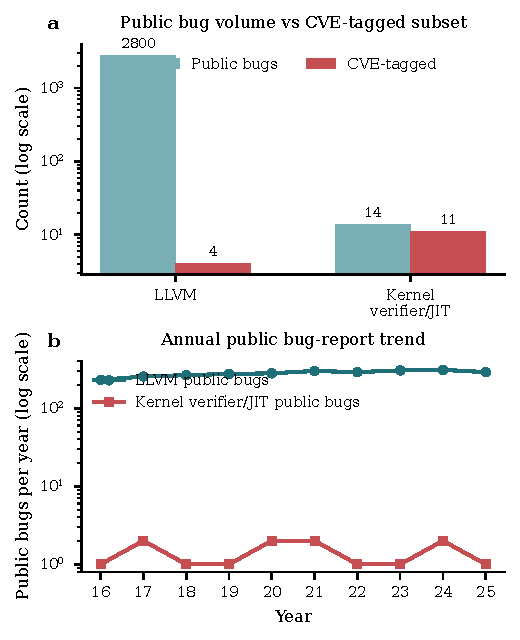
\includegraphics[width=\linewidth]{figures-next/motivation-security.pdf}
  \caption{Illustrative synthetic disclosure survey for the past decade. Panel (a) compares cumulative public bugs with the CVE-tagged subset: a large userspace compiler stack can accumulate thousands of ordinary bugs while only a tiny fraction are security-labeled, whereas a much smaller verifier/JIT bug population is far more likely to be treated as a security issue because it lies on the privileged kernel admission path. Panel (b) shows the corresponding annual report trend and emphasizes that the kernel-side population stays small but persistently security-sensitive. Example LLVM CVEs include CVE-2024-0151 and CVE-2024-7883; representative verifier/JIT issues include CVE-2017-16995, CVE-2020-8835, CVE-2021-29154, CVE-2021-31440, and CVE-2021-3490.}
  \label{fig:motivation-security}
\end{figure}
